% ==============================================================================
% Modelo para Especificação de Projeto de Software
% Prof. Vítor E. Silva Souza - NEMO/UFES :: DI/UFES :: PPGI/UFES
%
% Baseado em abtex2-modelo-trabalho-academico.tex, v-1.9.2 laurocesar
% Copyright 2012-2014 by abnTeX2 group at http://abntex2.googlecode.com/ 
%
% This work may be distributed and/or modified under the conditions of the LaTeX 
% Project Public License, either version 1.3 of this license or (at your option) 
% any later version. The latest version of this license is in
% http://www.latex-project.org/lppl.txt.
%
% IMPORTANTE:
% Instruções encontram-se espalhadas pelo documento. Para facilitar sua leitura,
% tais instruções são precedidas por (*) -- utilize a função localizar do seu
% editor para passar por todas elas.
% ==============================================================================

% Usa o estilo abntex2, configurando detalhes de formatação e hifenização.
\documentclass[
	12pt,				
	oneside,		
	a4paper,			
	english,			% Idioma adicional para hifenização.
	french,				% Idioma adicional para hifenização.
	spanish,			% Idioma adicional para hifenização.
	brazil				% O último idioma é o principal do documento.
	]{abntex2}


%%% Importação de pacotes. %%%

% Conserta o erro "No room for a new \count". 
% O comando \reserveinserts deve ser comentado ou não, dependendo da versão do LaTeX.
\usepackage{etex}
%\reserveinserts{28}

% Usa a fonte Latin Modern.
\usepackage{lmodern}

% Seleção de códigos de fonte.
\usepackage[T1]{fontenc}

% Codificação do documento em Unicode.
\usepackage[utf8]{inputenc}

% Usado pela ficha catalográfica.
\usepackage{lastpage}

% Indenta o primeiro parágrafo de cada seção.
\usepackage{indentfirst}

% Controle das cores.
\usepackage[usenames,dvipsnames]{xcolor}

% Inclusão de gráficos.
\usepackage{graphicx}

% Melhor controle de leiaute de tabelas.
\usepackage{tabularx}
\usepackage{colortbl}
\usepackage{longtable}
\usepackage{pdflscape}

% Inclusão de páginas em PDF diretamente no documento (para uso nos apêndices).
\usepackage{pdfpages}

% Para melhorias de justificação.
\usepackage{microtype}

% Citações padrão ABNT.
\usepackage[brazilian,hyperpageref]{backref}
\usepackage[alf]{abntex2cite}	
\renewcommand{\backrefpagesname}{Citado na(s) página(s):~}		% Usado sem a opção hyperpageref de backref.
\renewcommand{\backref}{}										% Texto padrão antes do número das páginas.
\renewcommand*{\backrefalt}[4]{									% Define os textos da citação.
	\ifcase #1
		Nenhuma citação no texto.
	\or
		Citado na página #2.
	\else
		Citado #1 vezes nas páginas #2.
	\fi}

% \rm is deprecated and should not be used in a LaTeX2e document
% http://tex.stackexchange.com/questions/151897/always-textrm-never-rm-a-counterexample
\renewcommand{\rm}{\textrm}

% Inclusão de símbolos não padrão.
\usepackage{amssymb}
\usepackage{eurosym}

% Para utilizar \eqref para referenciar equações.
\usepackage{amsmath}

% Permite mostrar figuras muito largas em modo paisagem com \begin{sidewaysfigure} ao invés de \begin{figure}.
\usepackage{rotating}

% Permite customizar listas enumeradas/com marcadores.
\usepackage{enumitem}

% Permite inserir hiperlinks com \url{}.
\usepackage{bigfoot}
\usepackage{hyperref}

% Permite usar o comando \hl{} para evidenciar texto com fundo amarelo. Útil para chamar atenção a itens a fazer.
\usepackage{soulutf8}

% Colorinlistoftodos package: to insert colored comments so authors can collaborate on the content.
% (*) Indicar o nome do aluno e substituir o nome do professor se for o caso.
\usepackage[colorinlistoftodos, textwidth=20mm, textsize=footnotesize]{todonotes}
\newcommand{\aluno}[1]{\todo[author=\textbf{Aluno},color=green!30,caption={},inline]{#1}}
\newcommand{\vitor}[1]{\todo[author=\textbf{Vítor},color=red!30,caption={},inline]{#1}}

% Permite inserir espaço em branco condicional (incluído no texto final só se necessário) em macros.
\usepackage{xspace}

% Permite incluir listagens de código com o comando \lstinputlisting{}.
\usepackage{listings}
\usepackage{caption}
\DeclareCaptionFont{white}{\color{white}}
\DeclareCaptionFormat{listing}{\colorbox{gray}{\parbox{\textwidth}{#1#2#3}}}
\captionsetup[lstlisting]{format=listing,labelfont=white,textfont=white}
\renewcommand{\lstlistingname}{Listagem}
\definecolor{mygray}{rgb}{0.5,0.5,0.5}
\lstset{
	basicstyle=\scriptsize,
	breaklines=true,
	numbers=left,
	numbersep=5pt,
	numberstyle=\tiny\color{mygray}, 
	rulecolor=\color{black},
	showstringspaces=false,
	tabsize=2,
    inputencoding=utf8,
    extendedchars=true,
    literate=%
    {é}{{\'{e}}}1
    {è}{{\`{e}}}1
    {ê}{{\^{e}}}1
    {ë}{{\¨{e}}}1
    {É}{{\'{E}}}1
    {Ê}{{\^{E}}}1
    {û}{{\^{u}}}1
    {ù}{{\`{u}}}1
    {â}{{\^{a}}}1
    {à}{{\`{a}}}1
    {á}{{\'{a}}}1
    {ã}{{\~{a}}}1
    {Á}{{\'{A}}}1
    {Â}{{\^{A}}}1
    {Ã}{{\~{A}}}1
    {ç}{{\c{c}}}1
    {Ç}{{\c{C}}}1
    {õ}{{\~{o}}}1
    {ó}{{\'{o}}}1
    {ô}{{\^{o}}}1
    {Õ}{{\~{O}}}1
    {Ó}{{\'{O}}}1
    {Ô}{{\^{O}}}1
    {î}{{\^{i}}}1
    {Î}{{\^{I}}}1
    {í}{{\'{i}}}1
    {Í}{{\~{Í}}}1
}




%%% Definição de variáveis. %%%
% (*) Substituir os textos abaixo com as informações apropriadas.
\titulo{SAGUP - Sistema de Administração e Gestão de Usuários e Permissões}
\autor{Gustavo Steim da Silveira}
\local{Vitória, ES}
\data{\the\year}
\instituicao{
	Universidade Federal do Espírito Santo -- UFES
	\par
	Centro Tecnológico
	\par
	Departamento de Informática}
\newcommand{\subtitulo}{Documento de Projeto de Sistema}
\newcommand{\versao}{1.0}

% Define a capa.
\renewcommand{\imprimircapa}{%
	\begin{capa}%
		\center
		
		{\ABNTEXchapterfont\large\subtitulo{}}
		\vfill
		\begin{center}
			\ABNTEXchapterfont\bfseries\LARGE\imprimirtitulo
		\end{center}
		
		\vfill
		\large\imprimirlocal
		\linebreak
		\large\imprimirdata
		\vspace*{1cm}
	\end{capa}
}

% Macros específicas do trabalho.
% (*) Inclua aqui termos que são utilizados muitas vezes e que demandam formatação especial.
% Exemplo: Java com TM (trademark) em superscript.
% Use sempre \xspace para que o LaTeX inclua espaço em branco após a macro somente quando necessário.
\newcommand{\java}{Java\texttrademark\xspace}




%%% Configurações finais de aparência. %%%

% Altera o aspecto de algumas cores.
\definecolor{blue}{RGB}{41,5,195}
\definecolor{lightgray}{gray}{0.9}

% Informações do PDF.
\makeatletter
\hypersetup{
	pdftitle={\@title}, 
	pdfauthor={\@author},
	pdfsubject={\imprimirpreambulo},
	pdfcreator={LaTeX with abnTeX2},
	pdfkeywords={abnt}{latex}{abntex}{abntex2}{trabalho acadêmico}, 
	colorlinks=true,				% Colore os links (ao invés de usar caixas).
	linkcolor=blue,					% Cor dos links.
	citecolor=blue,					% Cor dos links na bibliografia.
	filecolor=magenta,				% Cor dos links de arquivo.
	urlcolor=blue,					% Cor das URLs.
	bookmarksdepth=4
}
\makeatother

% Espaçamentos entre linhas e parágrafos.
\setlength{\parindent}{1.3cm}
\setlength{\parskip}{0.2cm}



%%% Páginas iniciais do documento: capa, folha de rosto, ficha, resumo, tabelas, etc. %%%

% Compila o índice.
\makeindex

% Inicia o documento.
\begin{document}

% Retira espaço extra obsoleto entre as frases.
\frenchspacing

% Inclui o brasão da UFES.
\begin{figure}[h]
  \centering
  
\includegraphics[scale=0.055]{brasao.jpg}
  \label{ppts3}
\end{figure} 

% Capa do trabalho.
\imprimircapa


% (*) Incluir linhas no registro de alterações a cada nova versão.
\begin{center}
	{\large\bfseries Registro de Alterações:}
	
	\vspace{0.5cm}
	\begin{tabular}{|c|p{45mm}|c|p{60mm}|} \hline
		
		\textbf{Versão} & \textbf{Responsável} & \textbf{Data}  & \textbf{Alterações} \\ \hline   
		
		1.0  & Gustavo Steim da Silveira & 27/05/2025 & Versão inicial. \\\hline 
	\end{tabular}
\end{center}
\newpage



%%% Início da parte de conteúdo do documento. %%%
% Marca o início dos elementos textuais.
\textual

% Inclusão dos capítulos como seções (sem quebra de página).
\begingroup
\let\clearpage\relax

\chapter{Introdução}
\label{sec-intro}
\vspace{-1cm}

Este documento apresenta o projeto (\textit{design}) do sistema \emph{SAGUP - Sistema de Administração e Gestão de Usuários e Permissões}. O SAGUP tem como principal objetivo oferecer uma plataforma segura, eficiente e acessível para o gerenciamento centralizado de usuários, seus respectivos perfis (roles) e permissões de acesso em sistemas corporativos.

O sistema permitirá realizar autenticação de usuários, cadastro e edição de perfis, atribuição de permissões específicas, bem como a visualização e auditoria de acessos. Essas funcionalidades são fundamentais para organizações que precisam garantir o controle rigoroso sobre quem pode acessar quais recursos, de forma auditável e escalável.

O SAGUP visa resolver lacunas frequentemente encontradas em sistemas legados ou soluções improvisadas, promovendo maior governança digital e conformidade com boas práticas de segurança da informação.

Além desta introdução, este documento está organizado da seguinte forma: 
a Seção~\ref{sec-plataforma} apresenta a plataforma de software utilizada na implementação do sistema;
a Seção~\ref{sec-rnfs} apresenta a especificação dos requisitos não funcionais (atributos de qualidade), definindo as táticas e o tratamento a serem dados aos atributos de qualidade considerados condutores da arquitetura; 
a Seção~\ref{sec-arquitetura} apresenta a arquitetura de software; por fim, 
a Seção~\ref{sec-frameweb} apresenta os modelos FrameWeb que descrevem os componentes da aplicação, com base na metodologia empregada.

\vspace*{1.5cm}

% ==============================================================================
% Projeto de Sistema - Nome do Aluno
% Capítulo 2 - Plataforma de Desenvolvimento
% ==============================================================================
\chapter{Plataforma de Desenvolvimento}
\label{sec-plataforma}
\vspace{-1cm}

Esta seção apresenta a plataforma de implementação adotada para o desenvolvimento do sistema \emph{SAGUP - Sistema de Administração e Gestão de Usuários e Permissões}. A arquitetura do sistema está baseada em um modelo cliente-servidor, com frontend desenvolvido em \textbf{Vue.js} e backend construído em \textbf{C\#}, utilizando o framework \textbf{ASP.NET Core}. A persistência de dados será feita através de um banco de dados relacional \textbf{SQLite}, com uso do \textbf{Entity Framework Core} para mapeamento objeto-relacional.

\begin{table}[H]
\centering
\caption{Plataforma de Desenvolvimento e Tecnologias Utilizadas}
\label{tabela-plataforma}
\begin{tabular}{|p{4.5cm}|p{7.5cm}|}
\hline
\textbf{Camada} & \textbf{Tecnologia / Ferramenta} \\
\hline
Frontend & Vue.js (versão 3), Quasar Framework \\
\hline
Backend & ASP.NET Core (C\#), .NET 7 \\
\hline
Persistência de Dados & SQLite \\
\hline
ORM & Entity Framework Core \\
\hline
API de Comunicação & RESTful APIs com JSON \\
\hline
Controle de Versão & GitHub \\
\hline
Gerenciamento de Dependências & NuGet (.NET), NPM (Node.js) \\
\hline
Ambiente de Desenvolvimento & Visual Studio, VS Code \\
\hline
Containerização (opcional) & Docker \\
\hline
\end{tabular}
\end{table}

A escolha dessas tecnologias visa garantir modernidade, escalabilidade, segurança e manutenibilidade para o sistema. O uso de Vue.js proporciona uma interface rica e reativa, enquanto o backend em C\# com ASP.NET Core oferece robustez e alto desempenho para a lógica de negócios e operações com dados.

\vspace*{1.5cm}

\chapter{Requisitos Não Funcionais}
\label{sec-rnfs}
\vspace{-1cm}

A Tabela~\ref{tabela-rnfs} apresenta a especificação dos requisitos não funcionais identificados no Documento de Especificação de Requisitos, os quais foram considerados condutores da arquitetura.

% Contador para IDs de Requisitos Não Funcionais.
% Substitua rnf-definir-label dentro dos \label{} abaixo por IDs do seu projeto.
\newcounter{rnfcount}
\renewcommand*\thernfcount{RNF-\arabic{rnfcount}}
\newcommand*\RNF{\refstepcounter{rnfcount}\thernfcount}
\setcounter{rnfcount}{0}

\begin{footnotesize}
\begin{longtable}{|r|p{13cm}|}
	\caption{Especificação de Requisitos Não Funcionais.}
	\label{tabela-rnfs}\\\hline
	
	\multicolumn{2}{|p{\dimexpr\linewidth-2\tabcolsep-2\arrayrulewidth}|}{\cellcolor{lightgray}\RNF\label{rnf-definir-label01} -- sentença descrevendo o RNF, conforme Documento de Especificação de Requisitos.}\\\hline
	
	Categoria: & \hl{Possíveis valores: Interoperabilidade, Segurança, Usabilidade, Eficiência, Confiabilidade, Disponibilidade, Manutenibilidade, Portabilidade.} \\\hline
	
	\parbox[t]{2cm}{\raggedleft Tática /\\Tratamento:} & \hl{Apontar a tática a ser usada e algum detalhe, quando pertinente sobre como essa tática será aplicada no contexto do projeto.} \\\hline
	
	Medida: & \hl{Medida a ser usada para estabelecer objetivamente um critério de aceitação para o atendimento do RNF.} \\\hline
	
	\parbox[t]{2cm}{\raggedleft Critério de\\Aceitação:} & \hl{Descrição do critério de aceitação. Deve permitir avaliar objetivamente se o RNF foi satisfeito ou não.} \\\hline
	
	% Linha em branco.
	\multicolumn{2}{c}{}\\\hline
	
	\multicolumn{2}{|p{\dimexpr\linewidth-2\tabcolsep-2\arrayrulewidth}|}{\cellcolor{lightgray}\RNF\label{rnf-definir-label02} -- sentença descrevendo o RNF, conforme Documento de Especificação de Requisitos.}\\\hline
	
	Categoria: & \hl{Possíveis valores: Interoperabilidade, Segurança, Usabilidade, Eficiência, Confiabilidade, Disponibilidade, Manutenibilidade, Portabilidade.} \\\hline
	
	\parbox[t]{2cm}{\raggedleft Tática /\\Tratamento:} & \hl{Apontar a tática a ser usada e algum detalhe, quando pertinente sobre como essa tática será aplicada no contexto do projeto.} \\\hline
	
	Medida: & \hl{Medida a ser usada para estabelecer objetivamente um critério de aceitação para o atendimento do RNF.} \\\hline
	
	\parbox[t]{2cm}{\raggedleft Critério de\\Aceitação:} & \hl{Descrição do critério de aceitação. Deve permitir avaliar objetivamente se o RNF foi satisfeito ou não.} \\\hline

\end{longtable}
\end{footnotesize}

\vspace*{1.5cm}

% ==============================================================================
% Projeto de Sistema - Gustavo Steim da Silveira
% Capítulo 4 - Arquitetura de Software
% ==============================================================================
\chapter{Arquitetura de Software}
\label{sec-arquitetura}
\vspace{-1cm} % Ajuste este espaçamento se necessário

O sistema \emph{\imprimirtitulo} foi desenvolvido seguindo a arquitetura clássica em camadas adotada por aplicações ASP.NET Core. Essa abordagem organiza a aplicação em módulos responsáveis por diferentes níveis de responsabilidade, promovendo a separação de interesses, reusabilidade e facilidade de manutenção.

\section{Visão Geral da Arquitetura em Camadas}

A Figura~\ref{figura-arquitetura-classica-dotnet} ilustra a arquitetura em camadas adotada no projeto. Essa estrutura compreende:

\begin{itemize}
    \item \textbf{Camada de Apresentação}: onde estão os controladores da API REST e, no frontend, os componentes Vue.js responsáveis pela interface com o usuário.
    \item \textbf{Camada de Aplicação}: que encapsula as regras de negócio por meio de serviços (Services) e objetos de transferência de dados (DTOs).
    \item \textbf{Camada de Domínio}: onde estão as entidades que representam os conceitos centrais do sistema.
    \item \textbf{Camada de Persistência}: que realiza o acesso ao banco de dados utilizando o Entity Framework Core.
\end{itemize}

\begin{figure}[H]
    \centering
    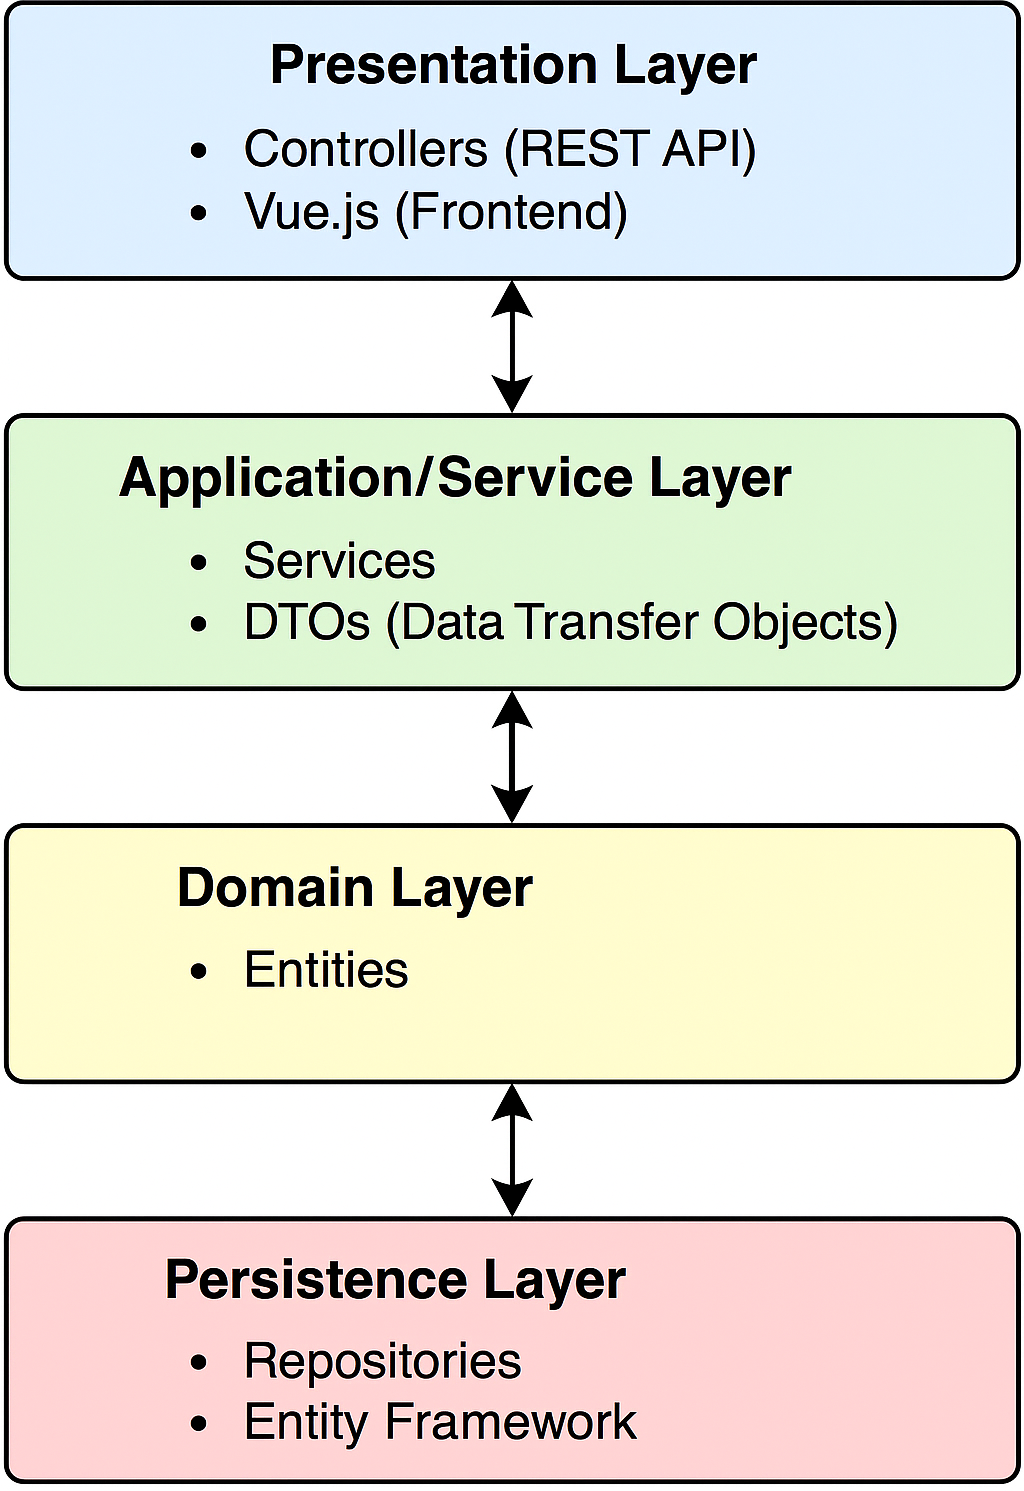
\includegraphics[width=0.9\textwidth]{figuras/arquitetura-dotnet-camadas.png}
    \caption{Arquitetura clássica em camadas do .NET}
    \label{figura-arquitetura-classica-dotnet}
\end{figure}

\section{Componentes do Sistema}

A seguir, apresentam-se os diagramas reais da implementação, agrupados conforme sua camada correspondente.

\subsection{Camada de Apresentação e Aplicação}

A Figura~\ref{figura-aplicacao} mostra os controladores e serviços responsáveis pelo fluxo da aplicação. As interfaces dos serviços (\textit{IUsuarioService}, \textit{IPerfilService}) são injetadas nos controladores seguindo o princípio de inversão de dependência.

\begin{figure}[H]
    \centering
    \includegraphics[width=\textwidth]{figuras/Aplicacao Class Diagram.png}
    \caption{Controladores, serviços e DTOs da aplicação}
    \label{figura-aplicacao}
\end{figure}

\subsection{Modelo de Domínio}

A Figura~\ref{figura-entidades} apresenta o modelo de entidades que representa os conceitos centrais do domínio, como usuários, perfis e permissões.

\begin{figure}[H]
    \centering
    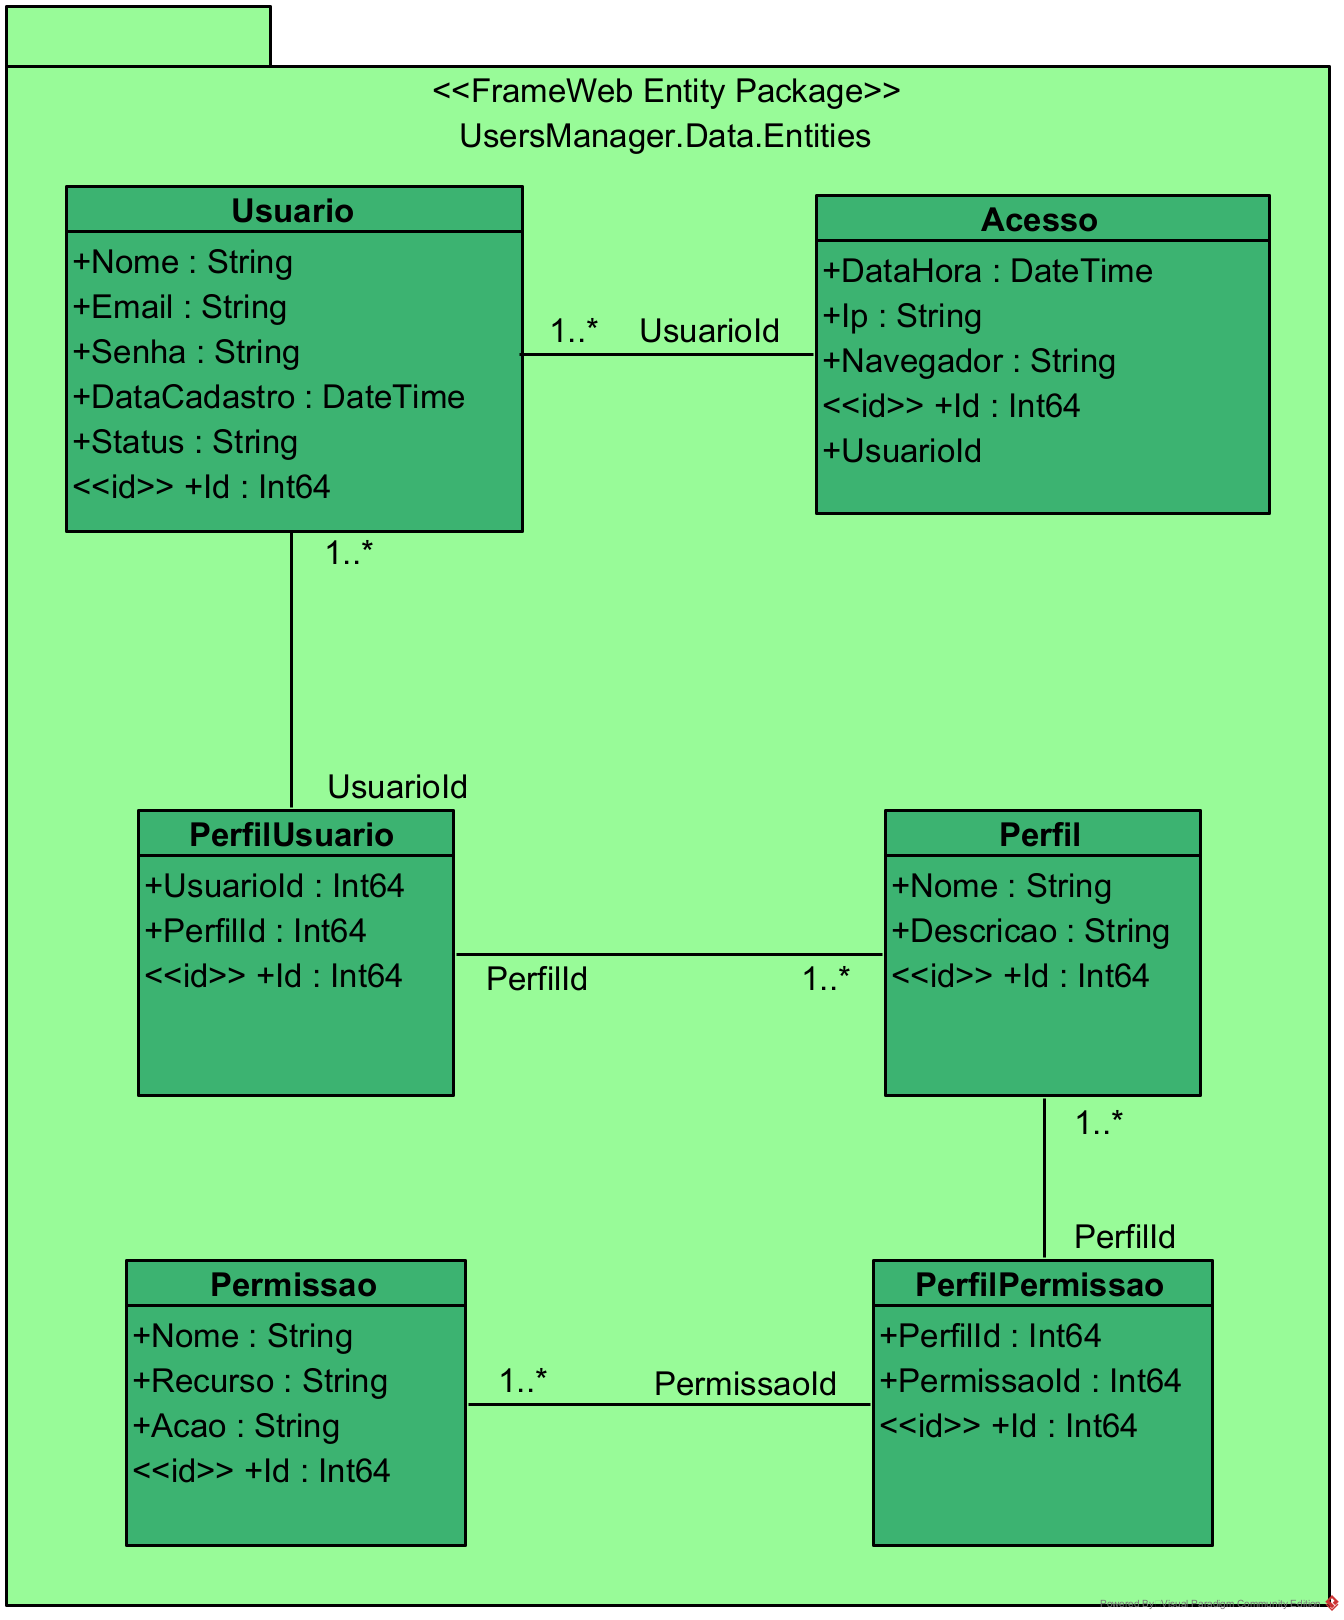
\includegraphics[width=0.8\textwidth]{figuras/Entidades Class Diagram.png}
    \caption{Entidades e relacionamentos do domínio}
    \label{figura-entidades}
\end{figure}

\subsection{Camada de Persistência}

A persistência é realizada via repositórios específicos para cada entidade, conforme ilustrado na Figura~\ref{figura-persistencia}. Esses componentes encapsulam as operações de consulta, inserção e atualização de dados utilizando o Entity Framework Core.

\begin{figure}[H]
    \centering
    \includegraphics[width=0.9\textwidth]{figuras/Persistencia Class Diagram.png}
    \caption{Repositórios e acesso a dados}
    \label{figura-persistencia}
\end{figure}

\section{Integração com o Frontend}

A comunicação entre o frontend Vue.js e o backend ASP.NET Core se dá por meio de requisições HTTP para a API RESTful. As figuras a seguir mostram os principais fluxos de navegação da aplicação:

\begin{itemize}
    \item Login: Figura~\ref{fig-navegacao-login}
    \item Edição de usuários: Figura~\ref{fig-navegacao-usuario}
    \item Gerenciamento de perfis: Figura~\ref{fig-navegacao-perfil}
    \item Dashboard: Figura~\ref{fig-navegacao-dashboard}
\end{itemize}

\begin{figure}[H]
    \centering
    \includegraphics[width=\textwidth]{figuras/Navegacao - Login.png}
    \caption{Navegação: processo de login}
    \label{fig-navegacao-login}
\end{figure}

\begin{figure}[H]
    \centering
    \includegraphics[width=\textwidth]{figuras/Navegacao - Edicao de Usuario.png}
    \caption{Navegação: edição de usuários}
    \label{fig-navegacao-usuario}
\end{figure}

\begin{figure}[H]
    \centering
    \includegraphics[width=\textwidth]{figuras/Navegacao - Edicao de Perfil.png}
    \caption{Navegação: gerenciamento de perfis e permissões}
    \label{fig-navegacao-perfil}
\end{figure}

\begin{figure}[H]
    \centering
    \includegraphics[width=\textwidth]{figuras/Navegacao - Ver Dashboard.png}
    \caption{Navegação: visualização do dashboard}
    \label{fig-navegacao-dashboard}
\end{figure}

\section{Considerações sobre Modelagem}

Embora o projeto utilize a arquitetura clássica do .NET, a modelagem inicial do sistema buscou inspiração em algumas diretrizes do FrameWeb, principalmente quanto à identificação de serviços e papéis das entidades no domínio. Para mais detalhes sobre a metodologia FrameWeb, consulte o projeto oficial\footnote{\url{https://nemo.inf.ufes.br/projetos/frameweb/}}.

% Referência ao FrameWeb (se usar bibtex ou manual)
% \bibitem{frameweb} Silva, C. A. et al. "FrameWeb: Uma abordagem orientada a modelos para aplicações Web baseadas em frameworks." Universidade Federal do Espírito Santo (UFES).


\vspace*{1.5cm}

% ==============================================================================
% Projeto de Sistema - Gustavo Steim da Silveira
% Capítulo 5 - FrameWeb
% ==============================================================================
\chapter{Modelagem FrameWeb}
\label{sec-frameweb}
\vspace{-1cm} % Ajuste este espaçamento se necessário

\emph{\imprimirtitulo} é um sistema Web cuja arquitetura utiliza o padrão em camadas, com tecnologias e \textit{frameworks} da plataforma .NET. Embora a abordagem FrameWeb tenha sido originalmente proposta com base em tecnologias Java (como JSF, CDI, JPA e JAAS), seus conceitos podem ser adaptados para outras plataformas, como demonstrado neste capítulo.

A Tabela~\ref{tabela-frameworks} apresenta a correspondência entre os tipos de \textit{frameworks} definidos pela abordagem FrameWeb e os utilizados no presente sistema. Em seguida, são apresentados os modelos FrameWeb para cada camada da arquitetura: Negócio, Acesso a Dados e Apresentação.

\begin{table}[H]
\centering
\caption{\textit{Frameworks} da arquitetura do sistema separados por categoria.}
\label{tabela-frameworks}
\begin{tabular}{|c|c|}
\hline
\textbf{Categoria de \textit{Framework}}& \textbf{\textit{Framework} Utilizado} \\\hline
Controlador Frontal & ASP.NET Core MVC \\\hline
Injeção de Dependências & Microsoft.Extensions.DependencyInjection \\\hline
Mapeamento Objeto/Relacional & Entity Framework Core \\\hline
Segurança & ASP.NET Identity \\\hline
\end{tabular}
\end{table}

\section{Camada de Negócio}
\label{sec-frameweb-negocio}

Nesta camada, o modelo de entidades e o modelo de aplicação foram representados conforme a abordagem FrameWeb. Embora o modelo do FrameWeb não tenha sido originalmente proposto para a plataforma .NET, os conceitos de \textbf{entidades de domínio} e \textbf{serviços de aplicação} foram mapeados diretamente para os componentes do sistema implementado.

\begin{figure}[H]
	\centering
	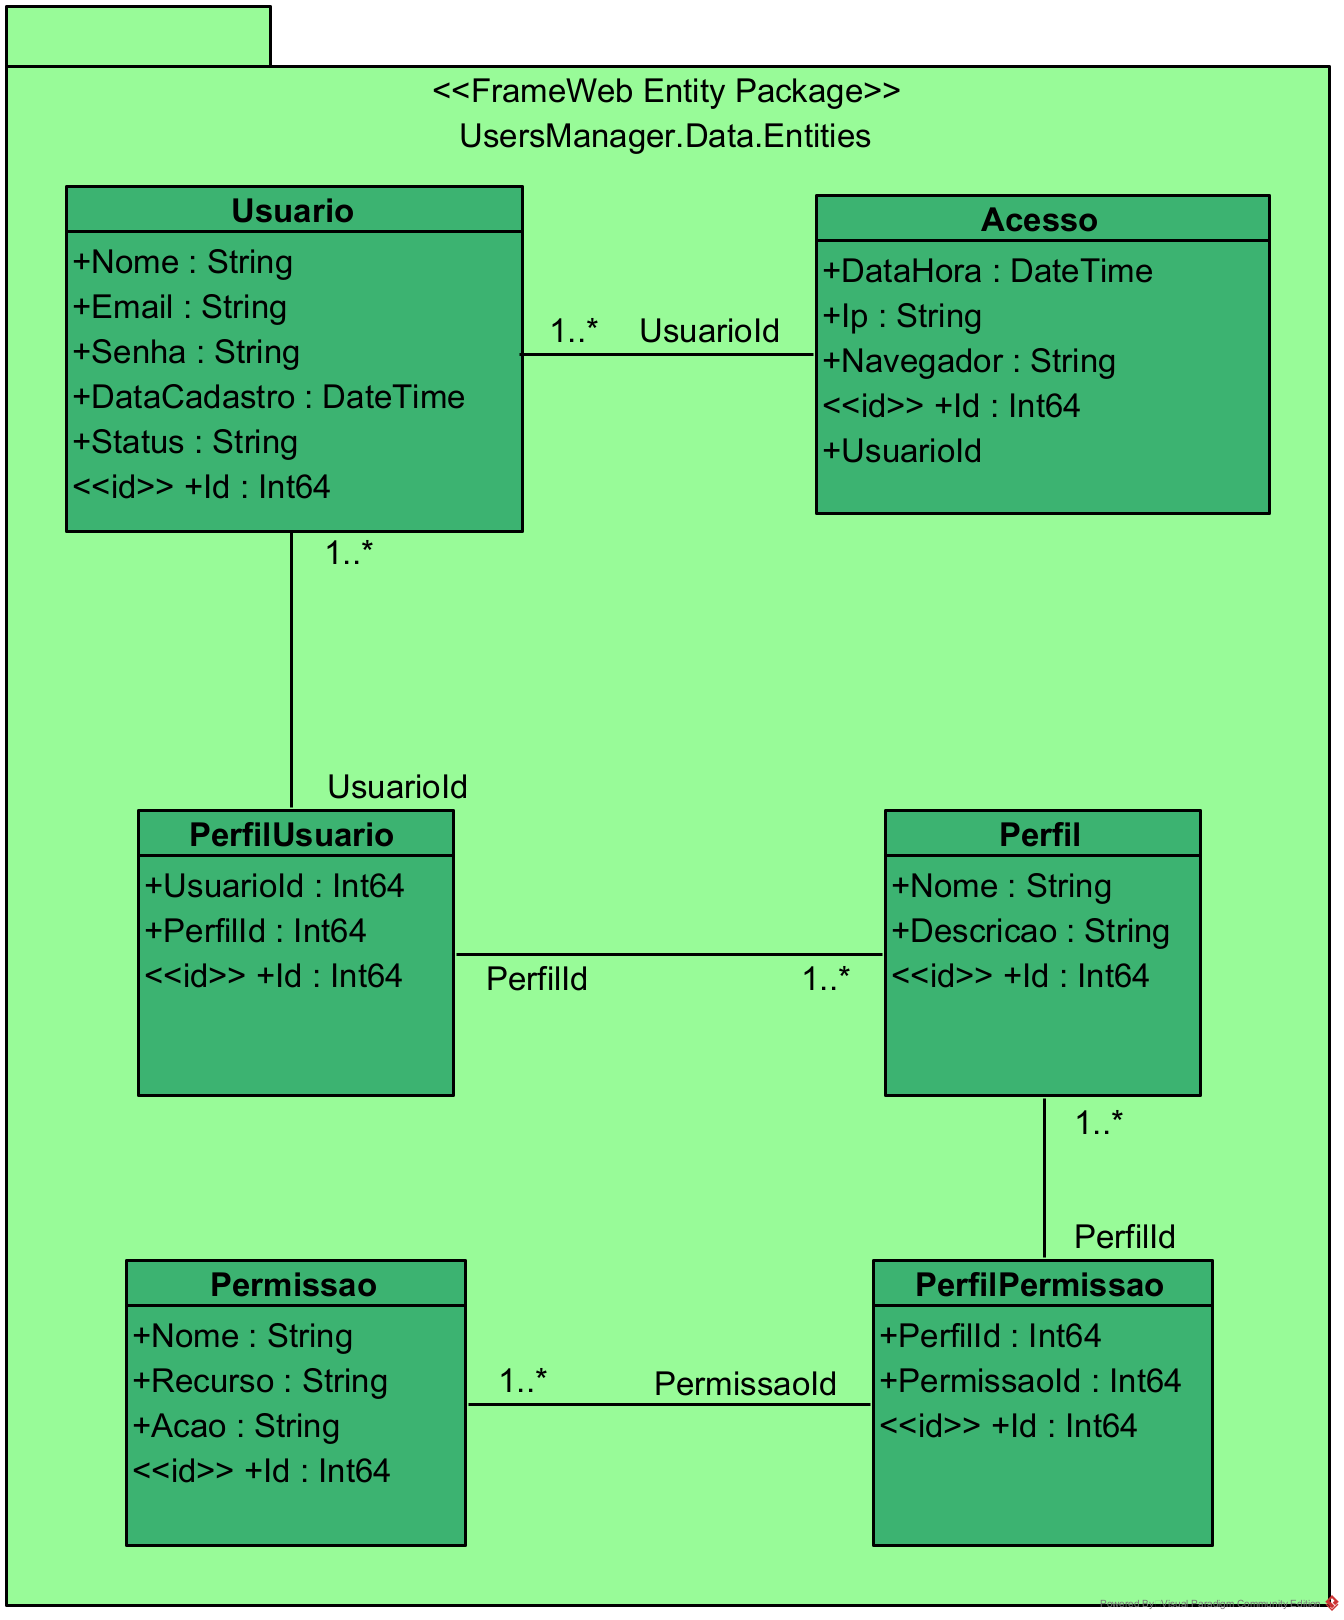
\includegraphics[width=0.95\textwidth]{figuras/Entidades Class Diagram.png}
	\caption{Modelo de Entidades adaptado para .NET}
	\label{fig:modelo-entidades}
\end{figure}

\begin{figure}[H]
	\centering
	\includegraphics[width=0.95\textwidth]{figuras/Aplicacao Class Diagram.png}
	\caption{Modelo de Aplicação adaptado para .NET}
	\label{fig:modelo-aplicacao}
\end{figure}

A principal adaptação aqui é a ausência de anotações específicas do Java (como \texttt{@Entity}, \texttt{@EJB}), substituídas por convenções e atributos do C\# e pelo uso de injeção de dependência nativa da plataforma.

\section{Camada de Acesso a Dados}
\label{sec-frameweb-dados}

A modelagem da camada de persistência também seguiu o modelo FrameWeb, representando os repositórios responsáveis por encapsular o acesso ao banco de dados. A principal diferença está no uso do \textbf{Entity Framework Core}, ao invés de JPA, e da \textbf{injeção de dependência} por meio do contêiner do ASP.NET.

\begin{figure}[H]
	\centering
	\includegraphics[width=0.9\textwidth]{figuras/Persistencia Class Diagram.png}
	\caption{Modelo de Persistência adaptado para .NET}
	\label{fig:modelo-persistencia}
\end{figure}

As interfaces e classes que implementam os repositórios foram modeladas conforme a abordagem recomendada para aplicações ASP.NET, respeitando a separação entre responsabilidades.

\section{Camada de Apresentação}
\label{sec-frameweb-apresentacao}

A modelagem da camada de apresentação também foi adaptada do modelo FrameWeb. Foram utilizados diagramas de navegação para representar os fluxos entre as páginas e os controladores, com base nas rotas configuradas no ASP.NET Core MVC.

\begin{figure}[H]
	\centering
	\includegraphics[width=0.9\textwidth]{figuras/Navegacao - Login.png}
	\caption{Navegação: Tela de Login}
	\label{fig:navegacao-login}
\end{figure}

\begin{figure}[H]
	\centering
	\includegraphics[width=0.9\textwidth]{figuras/Navegacao - Ver Dashboard.png}
	\caption{Navegação: Dashboard Principal}
	\label{fig:navegacao-dashboard}
\end{figure}

\begin{figure}[H]
	\centering
	\includegraphics[width=0.9\textwidth]{figuras/Navegacao - Edicao de Usuario.png}
	\caption{Navegação: Edição de Usuário}
	\label{fig:navegacao-edicao-usuario}
\end{figure}

\begin{figure}[H]
	\centering
	\includegraphics[width=0.9\textwidth]{figuras/Navegacao - Edicao de Perfil.png}
	\caption{Navegação: Edição de Perfil e Permissões}
	\label{fig:navegacao-edicao-perfil}
\end{figure}

Os controladores ASP.NET Core fazem o papel dos \textit{front controllers}, e os fluxos de navegação seguem a estrutura de rotas definida pelo framework.

\endgroup



%%% Páginas finais do documento: bibliografia e anexos. %%%
% Finaliza a parte no bookmark do PDF para que se inicie o bookmark na raiz e adiciona espaço de parte no sumário.
\phantompart

% Marca o início dos elementos pós-textuais.
\postextual

% Referências bibliográficas
\bibliography{bibliografia}

% Índice remissivo.
\phantompart
\printindex

% Fim do documento.
\end{document}
